\documentclass{article}
\newsavebox{\oldepsilon}
\savebox{\oldepsilon}{\ensuremath{\epsilon}}
\usepackage[minionint,mathlf,textlf]{MinionPro} % To gussy up a bit
\renewcommand*{\epsilon}{\usebox{\oldepsilon}}
\usepackage[margin=1in]{geometry}
\usepackage{graphicx} % For .eps inclusion
%\usepackage{indentfirst} % Controls indentation
\usepackage[compact]{titlesec} % For regulating spacing before section titles
\usepackage{adjustbox} % For vertically-aligned side-by-side minipages
\usepackage{array, amsmath,  mhchem}
\usepackage[hidelinks]{hyperref}
\usepackage{courier, subcaption}
\usepackage{multirow, enumerate}
\usepackage[autolinebreaks,framed,numbered]{mcode}
\usepackage{float}
\restylefloat{table}

\pagenumbering{gobble} 
\setlength\parindent{0 cm}
\renewcommand{\arraystretch}{1.2}
\begin{document}
\large

MCB 135 Problem Set 9 \hfill Due Wedesday, April 22, 2015 at 2:30 PM

\section*{Problem 1: Bicoid gradient scaling (40 points)}

The generic reaction-diffusion equation for a system with one component and one spatial dimension is\footnote{$\nabla^2$ is the Laplace operator. In one dimension, it is simply the second spatial derivative, $\partial_{xx}$. On the Cartesian plane, it is the sum of the two spatial derivatives, $\partial_{xx} + \partial_{yy}$.}:
\[ \frac{\partial}{\partial t} c(x,t) = f\left[ c(x,t) \right] + D \nabla^2  c(x,t) \]
When simulating such systems, we consider only a finite number of points on a one-dimensional grid.
\begin{enumerate}[a)]
\item Show, using the definition of the derivative, that the Laplacian term can be approximated on a grid with spacing $h$:
\[  \nabla^2 c(x,t) \approx  \frac{c(x-h,t) + c(x+h,t) - 2 \, c(x,t)}{h^2} \]
{\color{red}
\begin{eqnarray*}
\frac{\partial c}{\partial x} & \triangleq & \lim_{h \to 0} \frac{c(x+h,t) - c(x,t)}{h}\\
\frac{\partial^2 c}{\partial x^2} & = & \lim_{h \to 0} \frac{\partial}{\partial x} \left[ \frac{c(x+h,t) - c(x,t)}{h} \right]\\
& = & \lim_{h \to 0} \frac{\frac{c(x+h,t) - c(x,t)}{h} - \frac{c(x,t) - c(x-h,t)}{h}}{h} \\
& = & \lim_{h \to 0} \frac{c(x+h,t) + c(x-h,t) - 2 \, c(x,t)}{h^2}
\end{eqnarray*}
}
\end{enumerate}
We will model Bicoid reaction and diffusion in one dimension (representing the A-P axis of the embryo). Since Bicoid diffuses through the cytoplasm, it should not be able to ``exit" the embryo at either end: the boundaries of our grid must therefore be reflective. Unfortunately, the MATLAB function which implements the discrete Laplacian, \mcode{del2()}, does not handle these boundary conditions.
\begin{enumerate}[a)]
\setcounter{enumi}{1}
\item Write a function to estimate the discrete Laplacian on a grid with reflective boundaries at either end. The Turing pattern example script in the Lecture 29 notes, which implements the discrete Laplacian on a torus, may be a helpful starting point.

{\color{red}
Note how the reflective boundary is implemented in the script below by repeating the element at the edge. (This script also produces the plots for parts (c) and (d).).
}

\begin{lstlisting}
function [] = bicoid()
    L = 500; % Length of the embryo in microns
    D = 0.3; % Diffusion coefficient in square microns per second
    alpha = 10; % Rate of Bicoid translation in nM/s
    beta = 1 / (20 * 60); % Rate of Bicoid degradation in 1/s
    
    % Create a mesh of points for the reaction-diffusion system
    N = 100; % number of points on the grid
    h = L/N; % step size in microns
    x = zeros(1,N+1);
    
    % Determine how long the simulation will run and how frequently it will
    % update
    dt = 1; % 1 second
    t = 0;
    t_end = 2*60*60; % two hours
    
    for n = 1:round(t_end/dt)
        t = t+dt;
        x_right = x([2:N+1 N+1]);
        x_left = x([1 1:N]);
        x = x + dt * ( (D/h^2)*(x_left + x_right - 2 * x) - beta * x);
        x(1) = x(1) + dt * alpha; % Production only at the origin
    end
    plot([0:N]/N,x,'-k'); hold on;
    
    % Now repeat with a double-long embryp
    L = 1000; % Length of the embryo in microns
    N = 200; % step size remains 5 microns
    x = zeros(1,N+1);   
    for n = 1:round(t_end/dt)
        t = t+dt;
        x_right = x([2:N+1 N+1]);
        x_left = x([1 1:N]);
        x = x + dt * ( (D/h^2)*(x_left + x_right - 2 * x) - beta * x);
        x(1) = x(1) + dt * alpha;
    end
    plot([0:N]/N,x,'-r');
    
    % Finally, with an embryo half the normal length
    L = 250; % Length of the embryo in microns
    N = 50; % step size remains 5 microns
    x = zeros(1,N+1);
    for n = 1:round(t_end/dt)
        t = t+dt;
        x_right = x([2:N+1 N+1]);
        x_left = x([1 1:N]);
        x = x + dt * ( (D/h^2)*(x_left + x_right - 2 * x) - beta * x);
        x(1) = x(1) + dt * alpha; % Production only at the origin
    end
    plot([0:N]/N,x,'-b');
    
    set(gca,'YScale','log')
    xlabel('Fraction of body length')
    ylabel('Concentration (nM)')
    legend('Normal','Twice as long','Half as long','Location','SouthWest')
end
\end{lstlisting}

\item Suppose that the Bicoid protein gradient is established over the course of two hours in a 500 $\mu$m embryo according to the reaction-diffusion equation:
\[  \frac{\partial}{\partial t} c(x,t) =  \alpha \, \delta_k(x) - \beta \, c(x,t) + D \frac{\partial^2}{\partial x^2}  c(x,t) \]
where $\delta_k(x)$ is the Kronecker delta distribution, $\alpha$ = 10 nM/s is the translation rate, $\beta$ = 1/1800 s$^{-1}$ is the degradation rate, and $D$ = 0.3 $\mu$m$^2$/s is the diffusion rate. Show that the final Bicoid gradient is approximately exponential by simulating the system using  Euler's method and your subroutine from part (b). Assume that no Bicoid protein is present initially and use a step size\footnote{If you do use a different grid spacing, ensure that Bicoid is still synthesized in a 5 $\mu$m region.} of $h$=5 $\mu$m.

{\color{red}
A true exponential would appear as a straight line on these semi-log axes: with the exception of points far from the origin, the profile is as expected. (The gradient has simply not reached equilibrium yet: try extending the simulation to a ten-hour run time.)
}

\begin{center}
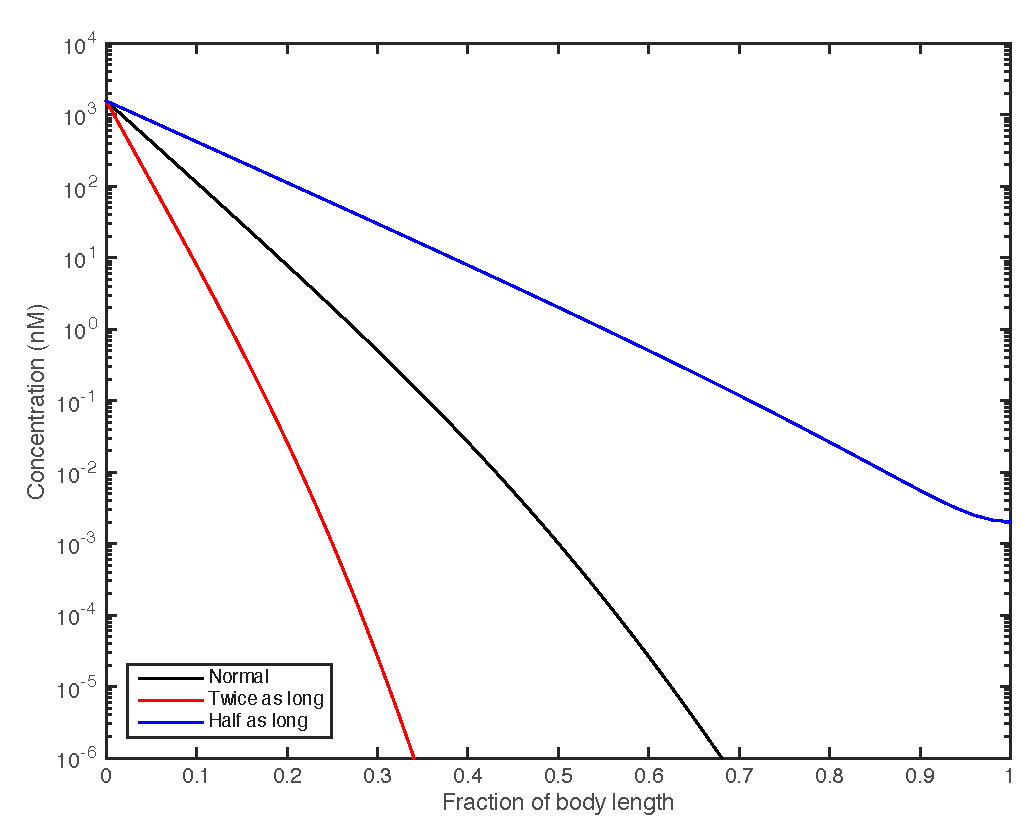
\includegraphics[width=0.5\textwidth]{prob1d.pdf}
\end{center}

\item Repeat for an embryo twice as long, and for a third embryo half as long as the original, maintaining the same step size and synthesis rate. Plot the Bicoid concentration profiles vs. fractional body length on the same axes. Does the concentration profile scale?\\

{\color{red}
See the plot above. The concentration profile does not scale.
}

\item Implement a gradient scaling mechanism of your choice and demonstrate an improvement by creating a plot similar to part (c) for comparison.\\

{\color{red}
Answers will vary. A quadratic degradation term converts the exponential gradient into a power law profile and is known to provide robustness against differences in production rate at the source (Eldar et al., 2003). For kicks we tested its ability to improve scaling here. The degradation term was changed from $-\beta x$ to $-\beta x^2$ in lines 22, 35, and 48. The resulting profile followed a power law as anticipated but did not improve the gradient scaling due to differences in embryo length.

\begin{center}
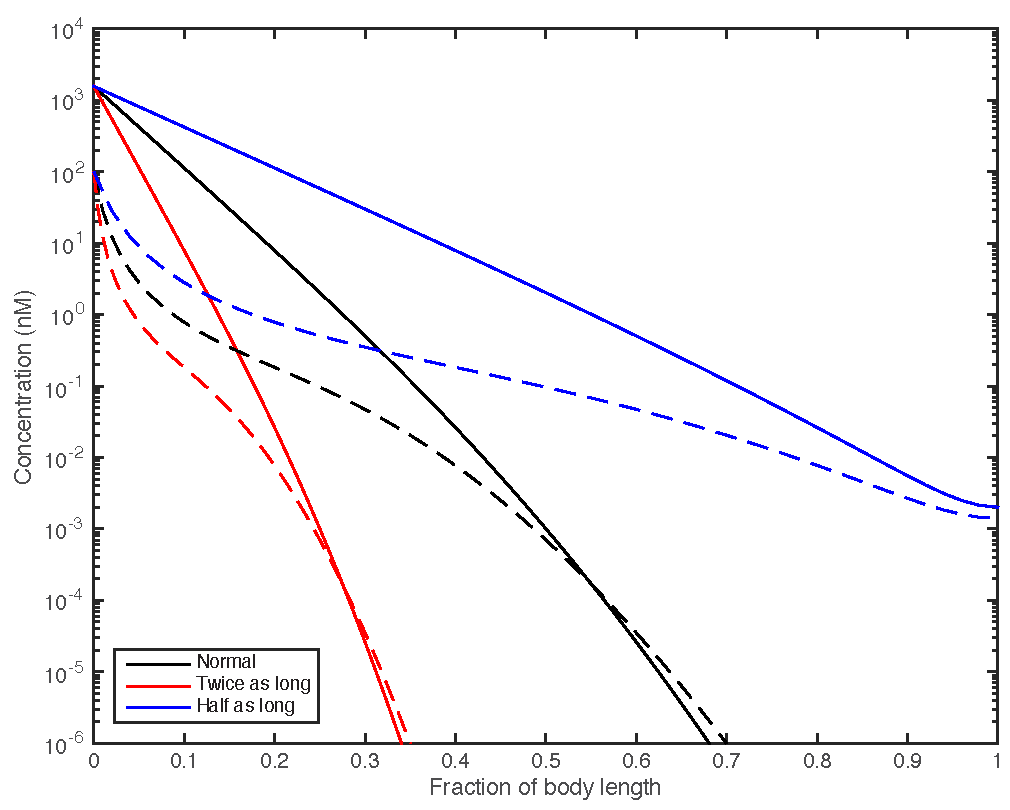
\includegraphics[width=0.45\textwidth]{prob1e.pdf} \hfill 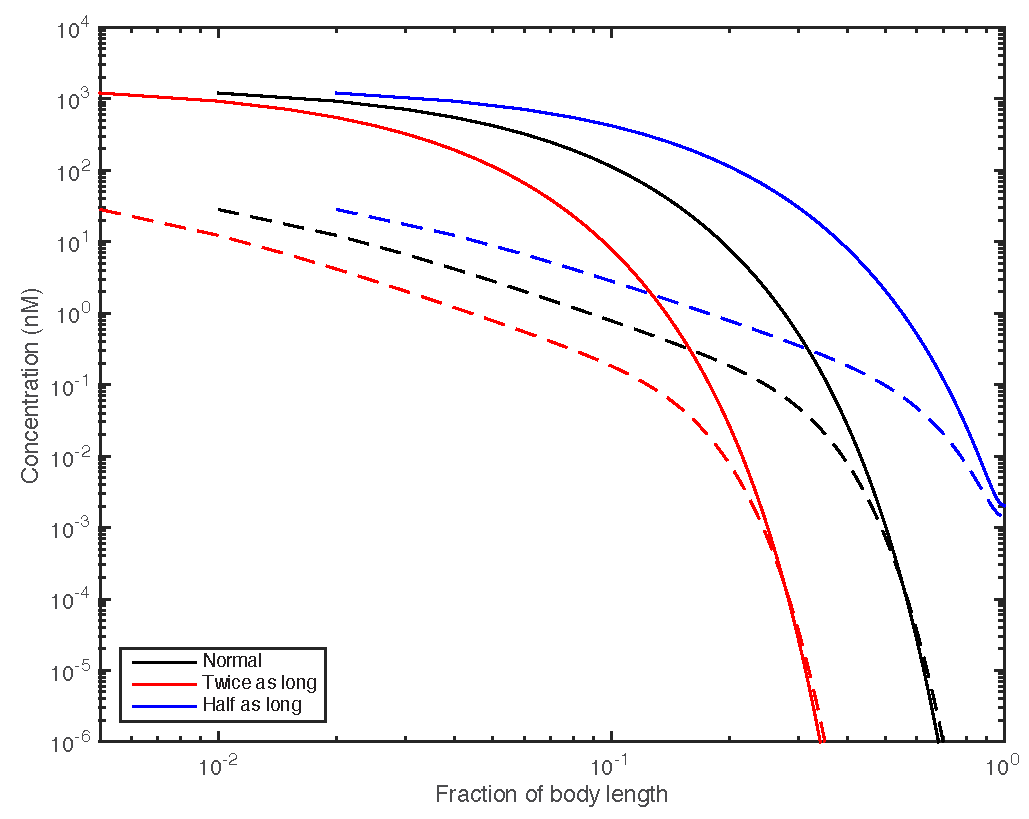
\includegraphics[width=0.45\textwidth]{prob1eloglog.pdf}
\end{center}


}

\end{enumerate}

\section*{Problem 2: Growing snake (60 points)}

Another Turing pattern mechanism proposed by Gierer and Meinhardt (1972) follows:
\[ \frac{\partial A}{\partial t} = \frac{\alpha \, A^2}{B} - \beta \, A + \epsilon \, D \,  \nabla^2 A \hspace{ 2 cm}  \frac{\partial B}{\partial t} = \gamma \, A^2  - \delta \, B + D \nabla^2 B\]
where all constants are positive. 
\begin{enumerate}[a)]
\item Show that the spatially-homogeneous solution for this system is:
\[ (A^*, B^*) = \left( \frac{\alpha \delta}{\beta \gamma}, \frac{\alpha^2 \delta}{\beta^2 \gamma} \right) \]
{ \color{red}
\begin{eqnarray*}
\frac{\partial A}{\partial t} = 0: & & \frac{\alpha A^{*2}}{B^*} - \beta \, A^* = 0\\
& \implies & A^* = \frac{\beta B^*}{\alpha}\\
\frac{\partial B}{\partial t} = 0: & & \gamma \left( \frac{\beta B^*}{\alpha} \right)^2- \delta \, B^* = 0\\
& \implies & B^* = \frac{\alpha^2 \, \delta}{\beta^2 \, \gamma}\\
& \implies & A^* = \frac{\alpha \, \delta}{\beta \, \gamma}
\end{eqnarray*}
}
\item Show that for Turing patterns to arise, the following two conditions must hold:
\[ \delta > \beta \hspace{2 cm} \textrm{ and } \hspace{2 cm} \left( \beta + \delta \, \epsilon \right)^2  > 8 \, \beta \, \delta \, \epsilon \]
{\color{red}
First, calculate the Jacobian:
\[ \mathbf{C} = \begin{pmatrix} \frac{2\alpha A}{B} - \beta & -\frac{\alpha A^2}{B^2} \\ 2\gamma A & - \delta \end{pmatrix}_{(A^*,B^*)} = \begin{pmatrix} \beta & -\frac{\beta^2}{\alpha} \\ \frac{2 \alpha \delta}{\beta} & - \delta \end{pmatrix}  \]
The requirement that the fixed point be stable in the absence of diffusion places a constraint on the trace of $\mathbf{C}$:
\[ c_{11} + c_{22} < 0 \implies \beta - \delta < 0 \implies \delta > \beta \]
The requirement that the fixed point be unstable in the presence of diffusion places constraints on the relationship between the diffusion coefficients and the terms of the Jacobian:
\begin{eqnarray*}
\frac{c_{11}}{D_A} - \frac{c_{22}}{D_B} & > & 2 \sqrt{\left| \frac{c_{12}}{D_A}  \right|\left| \frac{c_{21}}{D_B}  \right|}\\
\frac{\beta}{\epsilon \, D} + \frac{\delta}{D} & > & 2 \sqrt{\left| \frac{- \beta^2}{\alpha \, \epsilon \, D}  \right|\left| \frac{2 \, \alpha \, \delta }{\beta \, D}  \right|} = 2 \sqrt{\frac{2 \, \beta \, \delta}{ \epsilon \, D^2} }\\
 \beta + \delta \, \epsilon  & > & 2 \sqrt{2 \, \beta \, \delta \, \epsilon } \\
 \left( \beta + \delta \, \epsilon \right)^2 & > & 8 \, \beta \, \delta \, \epsilon
\end{eqnarray*}


}
\end{enumerate}
Consider the specific case where $\alpha=\beta =\gamma = 1$, $\delta = 1.1$, $\epsilon = 0.12$, and $D=15$. You will use Euler's method to simulate this system on a two-dimensional grid representing the skin of a snake. The left and right boundaries of the grid (the ``head" and ``tail") should be reflective under diffusion, while the top and bottom should wrap around. You may wish to modify the example Turing pattern script on the course website for this purpose.
\begin{enumerate}[a)]
\setcounter{enumi}{3}
\item Simulate this system on a grid with dimensions 5 units x 10 units (a ``baby snake"). Use a step size of one unit; choose the time step and duration appropriately to allow the system to reach its steady-state pattern. Include an image of your results. How many stripes does this snake have?\\
\begin{center}

\includegraphics[width=0.05\textwidth]{prob2d.pdf}
\end{center}

{\color{red}
The snake has one stripe (and it is perpendicular to its body axis). The code below will be used in parts (e-f) with only $N_1$ and $N_2$ changing.
}

\begin{lstlisting}
function [] = findstripes_reflective()
    % Create a mesh of spatial points for the reaction-diffusion system
    N1 = 5;
    N2 = 10;
    h = 1;
    [xx,yy] = meshgrid([0:N2], [0:N1]);
    
    % Determine how long the simulation will run and how frequently it will
    % update
    dt = .01;
    t = 0;
    t_end = 1000;
    
    % System parameters for spots
    alpha = 1;
    beta = 1;
    gamma = 1;
    delta = 1.1;
    D = 15;
    epsilon = 0.12; % 0.1 was original
    
    % initiate the system near the fixed point, but with small added noise
    A = ((alpha*delta)/(beta*gamma))*ones(size(xx)) + 0.1*randn(size(xx)); 
    B = (alpha^2 * delta/(gamma* beta^2))*ones(size(xx)) + 0.1*randn(size(xx)); 
    
    for n = 1:round(t_end/dt)
        t = t+dt;
        
        % Calculate the discrete Laplacian assuming the field is toroidal.
        AE = A(:,[2:N2+1 N2+1]);
        AW = A(:,[1 1:N2]);
        AN = A([N1+1 1:N1],:);
        AS = A([2:N1+1 1],:);
        BE = B(:,[2:N2+1 N2+1]);
        BW = B(:,[1 1:N2]);
        BN = B([N1+1 1:N1],:);
        BS = B([2:N1+1 1],:);
        A = A + dt * (-1 * beta * A + (alpha * A.^2)./B ) + dt * epsilon * D * (AE+AW+AN+AS-4*A)/h^2;
        B = B + dt * (gamma * A.^2 - delta * B) + dt * D * (BE+BW+BN+BS-4*B)/h^2;
    end
    
    % Display the image
    Ascaled = (A - min(min(A))) ./ (max(max(A)) - min(min(A)));
    imshow(Ascaled)
end
\end{lstlisting}

\item The snake grows up. Repeat the simulation on a grid with dimensions 10 units by 100 units. How many stripes does the snake have now? Include an image of the results.

\begin{center}

\includegraphics[width=0.5\textwidth]{prob2e.pdf}
\end{center}

{\color{red}
This snake has about 6-7 stripes.
}

\item The snake lives large. Repeat on a grid with dimensions 100 units by 100 units. Include an image of the results.

\begin{center}

\includegraphics[width=0.5\textwidth]{prob2f.pdf}
\end{center}

{\color{red}
The snake got so fat that it is now spotted. The average number of spots from left to right in any row appears to have also gone up slightly.
}

\item Determine which modes are unstable for organisms with the following lengths (i) $L=\sqrt{5^2 + 10^2}$, (ii) $L=\sqrt{10^2 + 100^2}$, and (iii) $L=\sqrt{100^2 + 100^2}$. How are these values reflected in the images you produced in (d-f)? Hint: see Iglesias section 3.3.2 and Figure 3.9 for a worked example.

\begin{center}
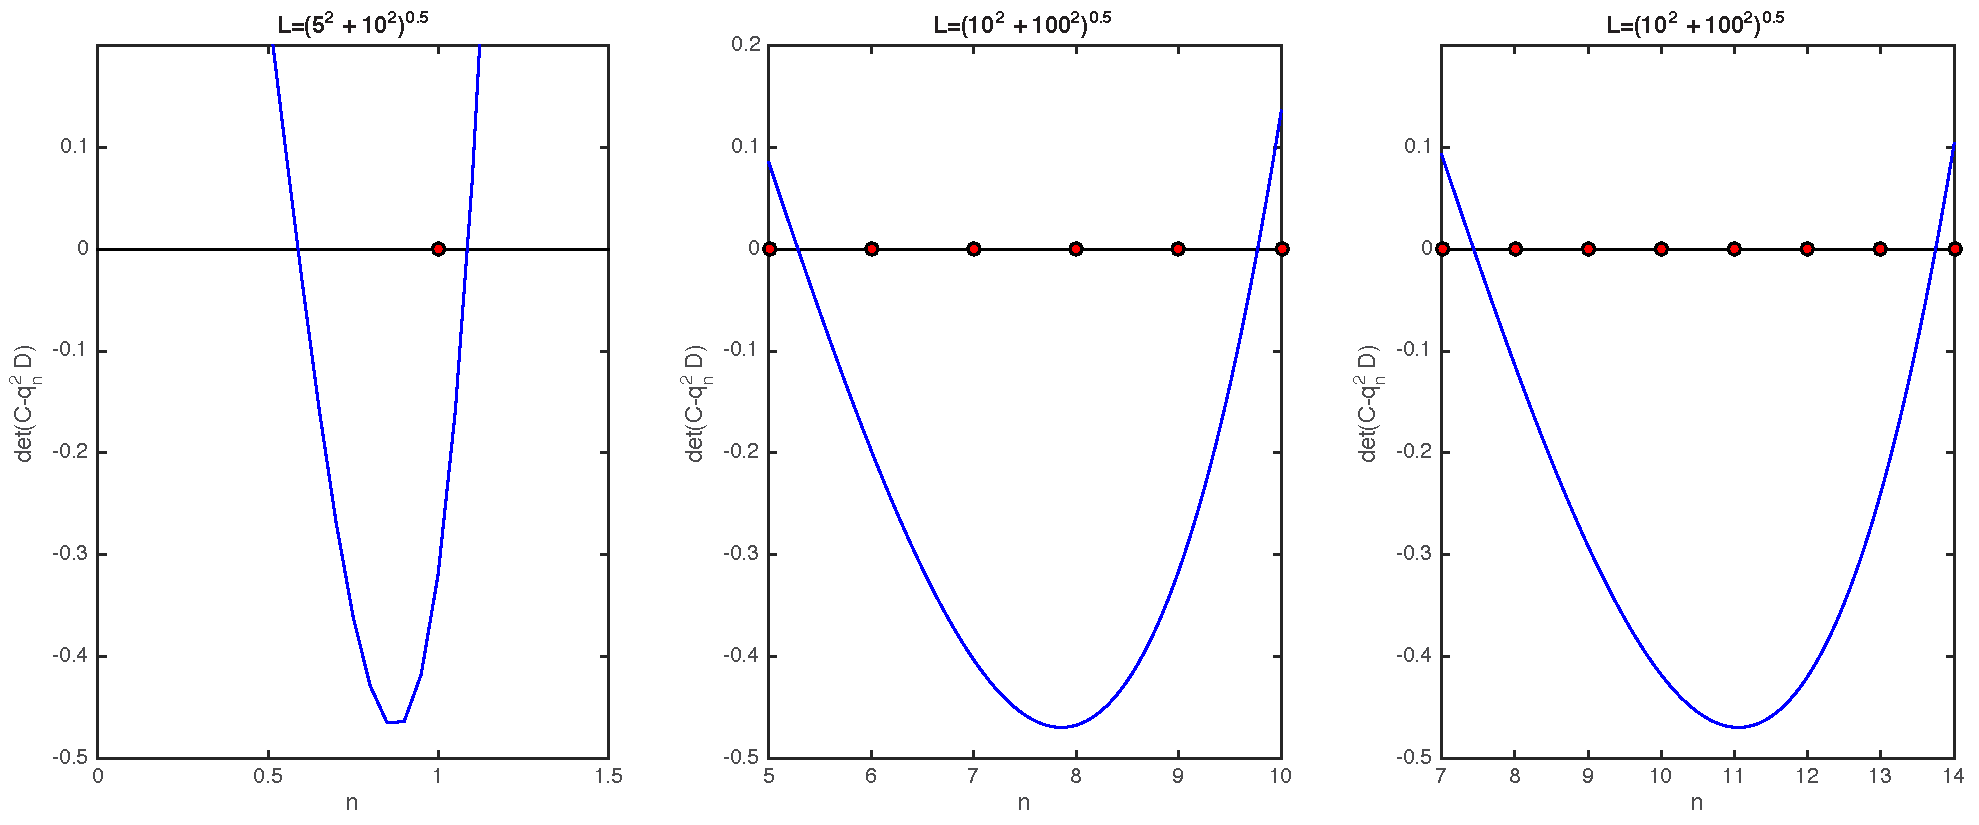
\includegraphics[width=0.8\textwidth]{unstable_nodes.pdf}
\end{center}

{\color{red}
Unstable modes have $q_n = 2\pi n/L$ which satisfies:
\[ \left| \mathbf{C} - q_n^2 \mathbf{D} \right| = c_{11}c_{22} - c_{12} c_{21}  - q_n^2 \left( c_{11} D_B + c_{22} D_A \right) + q_n^4 D_A D_B < 0 \]
To find them, plot the quadratic vs. $n$, then find the whole number values of $n$ within the region where the graph is less than zero. There is only one mode for the smallest value of $L$, consistent with the fact that a field of this size gave only one stripe. Similarly the seven stripes observed for the second snake falls squarely within the permissive region for the second value of $L$, and so forth.\\

To understand the behavior in the widest region, we ought to have used a form of perturbation that would produce two-dimensional standing waves. This approach was not required for credit; a sketch of the approach is presented in lecture 30 for those interested.
}

\begin{lstlisting}
function [] = unstable_modes()
    % These constants do not change
    D = 15;
    epsilon = 0.12;
    c11 = 1;
    c12 = -1;
    c21 = 2.2;
    c22 = -1.1;
    det_C = c11*c22 - c12 * c21;
    figure
    
    % Plot for smallest snake
    x = 0:0.05:1.5;
    n = 1;
    L = (5^2 + 10^2)^0.5;
    q_x = (2*pi/L) .* x;
    q_n = (2*pi/L) .* n;
    
    subplot(1,3,1)
    y_x = det_C - (c11*D + c22*D*epsilon) .* q_x.^2 + (epsilon * D^2) .* q_x.^4; 
    plot([0, 1.5],[0 0],'-k'); hold on;
    plot(x,y_x, '-b')
    plot(n,[0], 'or', 'MarkerFaceColor', [1 0 0], 'MarkerEdgeColor', [0 0 0])
    title('L=(5^2 + 10^2)^{0.5}')
    xlabel('n')
    ylabel('det(C-q_n^2 D)')
    axis([0 1.5 -0.5 0.2])
    
    % Plot for adult snake
    x = 5:0.05:10;
    n = 5:10;
    L = (10^2 + 100^2)^0.5;
    q_x = (2*pi/L) .* x;
    q_n = (2*pi/L) .* n;
    
    subplot(1,3,2)
    y_x = det_C - (c11*D + c22*D*epsilon) .* q_x.^2 + (epsilon * D^2) .* q_x.^4; 
    plot([5, 10],[0 0],'-k'); hold on;
    plot(x,y_x, '-b')
    plot(n,[0], 'or', 'MarkerFaceColor', [1 0 0], 'MarkerEdgeColor', [0 0 0])
    title('L=(10^2 + 100^2)^{0.5}')
    xlabel('n')
    ylabel('det(C-q_n^2 D)')
    
    % Plot for fat snake
    x = 7:0.05:14;
    n = 7:14;
    L = (100^2 + 100^2)^0.5;
    q_x = (2*pi/L) .* x;
    q_n = (2*pi/L) .* n;
    
    subplot(1,3,3)
    y_x = det_C - (c11*D + c22*D*epsilon) .* q_x.^2 + (epsilon * D^2) .* q_x.^4; 
    plot([7, 14],[0 0],'-k'); hold on;
    plot(x,y_x, '-b')
    plot(n,[0], 'or', 'MarkerFaceColor', [1 0 0], 'MarkerEdgeColor', [0 0 0])
    title('L=(10^2 + 100^2)^{0.5}')
    xlabel('n')
    ylabel('det(C-q_n^2 D)')
    axis([7 14 -0.5 0.2])
end
\end{lstlisting}

\end{enumerate}

\end{document}